\chapter{Methodology}

\label{Chapter4}

\section{Baseline and Its Limitations}
\label{sec:baseline-elasticity-simulation}

The predictive baseline is a LightGBM regressor trained to forecast weekly units sold. It uses the pre-pricing commercial context and the discount rate (\texttt{discount}) as the price-related input. Discounted price (\texttt{actual\_price}) is excluded from this baseline so that the simulated price-response curve is driven by discount, matching the original operational setup evaluated in this project. Predictive quality is evaluated with WMAPE, the same metric used internally for demand planning.

The diagnostic follows the markdown-curve logic introduced in Section~\ref{sec:local-effects-markdown-curves}. For each reference-week, predictions are simulated over the operational discount grid while the remaining context is held fixed. Sales are normalized at the 20\% reference discount and compared with the break-even curve.

\begin{figure}[h]
\centering
\IfFileExists{Figures/baseline_curve.png}{
\includegraphics[width=0.82\textwidth]{baseline_curve}}{\fbox{\parbox{0.82\textwidth}{\centering Add \texttt{baseline\_curve.png} to the \texttt{Figures} folder.}}}
\caption{Predictive LightGBM simulation for a representative reference-week. Sales multipliers are normalized at the 20\% discount and compared with the break-even multiplier.}
\label{fig:baseline-curve}
\end{figure}

Across the holdout season, the predictive simulation tends to recommend the minimum allowed discount, which is the lowest boundary. This suggests that accurate demand forecasting alone is not enough for markdown optimization, because simulated price changes may still reflect the historical markdown policy.

In the data, deeper discounts are often assigned to weaker or overstocked references, so the observed price-sales relationship is confounded. This motivates the causal reformulation developed in Chapter~\ref{Chapter3}. Baseline simulation details and hyperparameters are reported in Appendix~\ref{AppendixA}.


\section{Specification and DML Setup}
\label{sec:specification-dml}

The final causal model uses season-normalized weekly demand, defined in Chapter~\ref{Chapter2}, transformed into logarithms. The treatment is discounted price, corresponding to \texttt{actual\_price}. Let $i$ denote one reference-week observation. The base DML specification is

\begin{equation}
\log(Q_i) = \beta P_i + g(X_i) + \varepsilon_i.
\label{eq:final_spec}
\end{equation}

where $Q_i$ is season-normalized weekly demand, $P_i$ is discounted price, and $X_i$ contains the pre-pricing covariates for that reference-week.

Because only demand is logged, $\beta$ is a semi-elasticity. A one-euro increase in price changes expected demand by approximately $100\beta$ percent. Since demand should fall when price increases, $\beta$ is expected to be negative. For the revenue derivation, define $\eta=-\beta>0$.

The functional form matters because it determines the shape of the implied revenue curve. A log-log demand model has the form

\begin{equation}
Q(P)=AP^{-\eta},
\end{equation}

where $P$ is price and $\eta>0$ is the price elasticity. Revenue is then

\begin{equation}
R(P)=P Q(P)=AP^{1-\eta}.
\end{equation}

This function is monotonic unless $\eta=1$: if $\eta>1$, revenue decreases with price; if $\eta<1$, revenue increases with price. Therefore, over a bounded markdown grid, the optimum tends to fall at one of the boundaries.

By contrast, a log-linear demand model has the form

\begin{equation}
Q(P)=Ae^{-\eta P}.
\end{equation}

Revenue is

\begin{equation}
R(P)=P Q(P)=APe^{-\eta P}.
\end{equation}

This revenue curve can have an interior maximum at

\begin{equation}
P^*=\frac{1}{\eta},
\end{equation}

provided that $P^*$ lies within the feasible price grid. This is useful for markdown optimization because it allows smoother curves and does not mechanically push the optimizer to the lowest or highest discount.

The treatment is encoded as discounted price rather than the discount rate. The discounted price is computed as

\begin{equation}
P_i(d)=P_i^{0}(1-d),
\end{equation}

where $P_i^{0}$ is the original price of reference-week $i$ and $d$ is the discount rate. Although discount rate is operationally relevant, revenue is directly computed as price times quantity. The discounted price is therefore the natural scale for the optimization problem.

This distinction is also important when comparing different items. For example, a five-percentage-point discount change represents a different cash value for a low-price product than for a high-price product. Using discounted price keeps the treatment in euros and aligns it with the revenue objective.

The confounder set $X$ contains 19 pre-pricing variables observed at the three-week anchor. These include calendar information, product-family indicators, original price level, season performance, normalized sales and stock indicators, pre-sale demand signals, coverage measures, and material-composition variables when available. The original price remains in $X$ because it captures product price tier. The discount rate is excluded because it is mechanically related to discounted price and original price; including it would partially control away the treatment variation of interest.

DML fits two LightGBM nuisance models: $\hat{l}(X)$ for logged normalized demand and $\hat{m}(X)$ for discounted price. Residuals are computed as

\begin{equation}
\tilde{Y}_i = Y_i - \hat{l}(X_i),
\qquad
\tilde{T}_i = T_i - \hat{m}(X_i).
\end{equation}

Cross-fitting is leave-one-season-out to prevent temporal and within-sample leakage. The nuisance hyperparameters are reported in Appendix~\ref{AppendixA}.

\begin{figure}[htbp]
\centering
\IfFileExists{Figures/dml_residualized_treatment_outcome_linear.png}{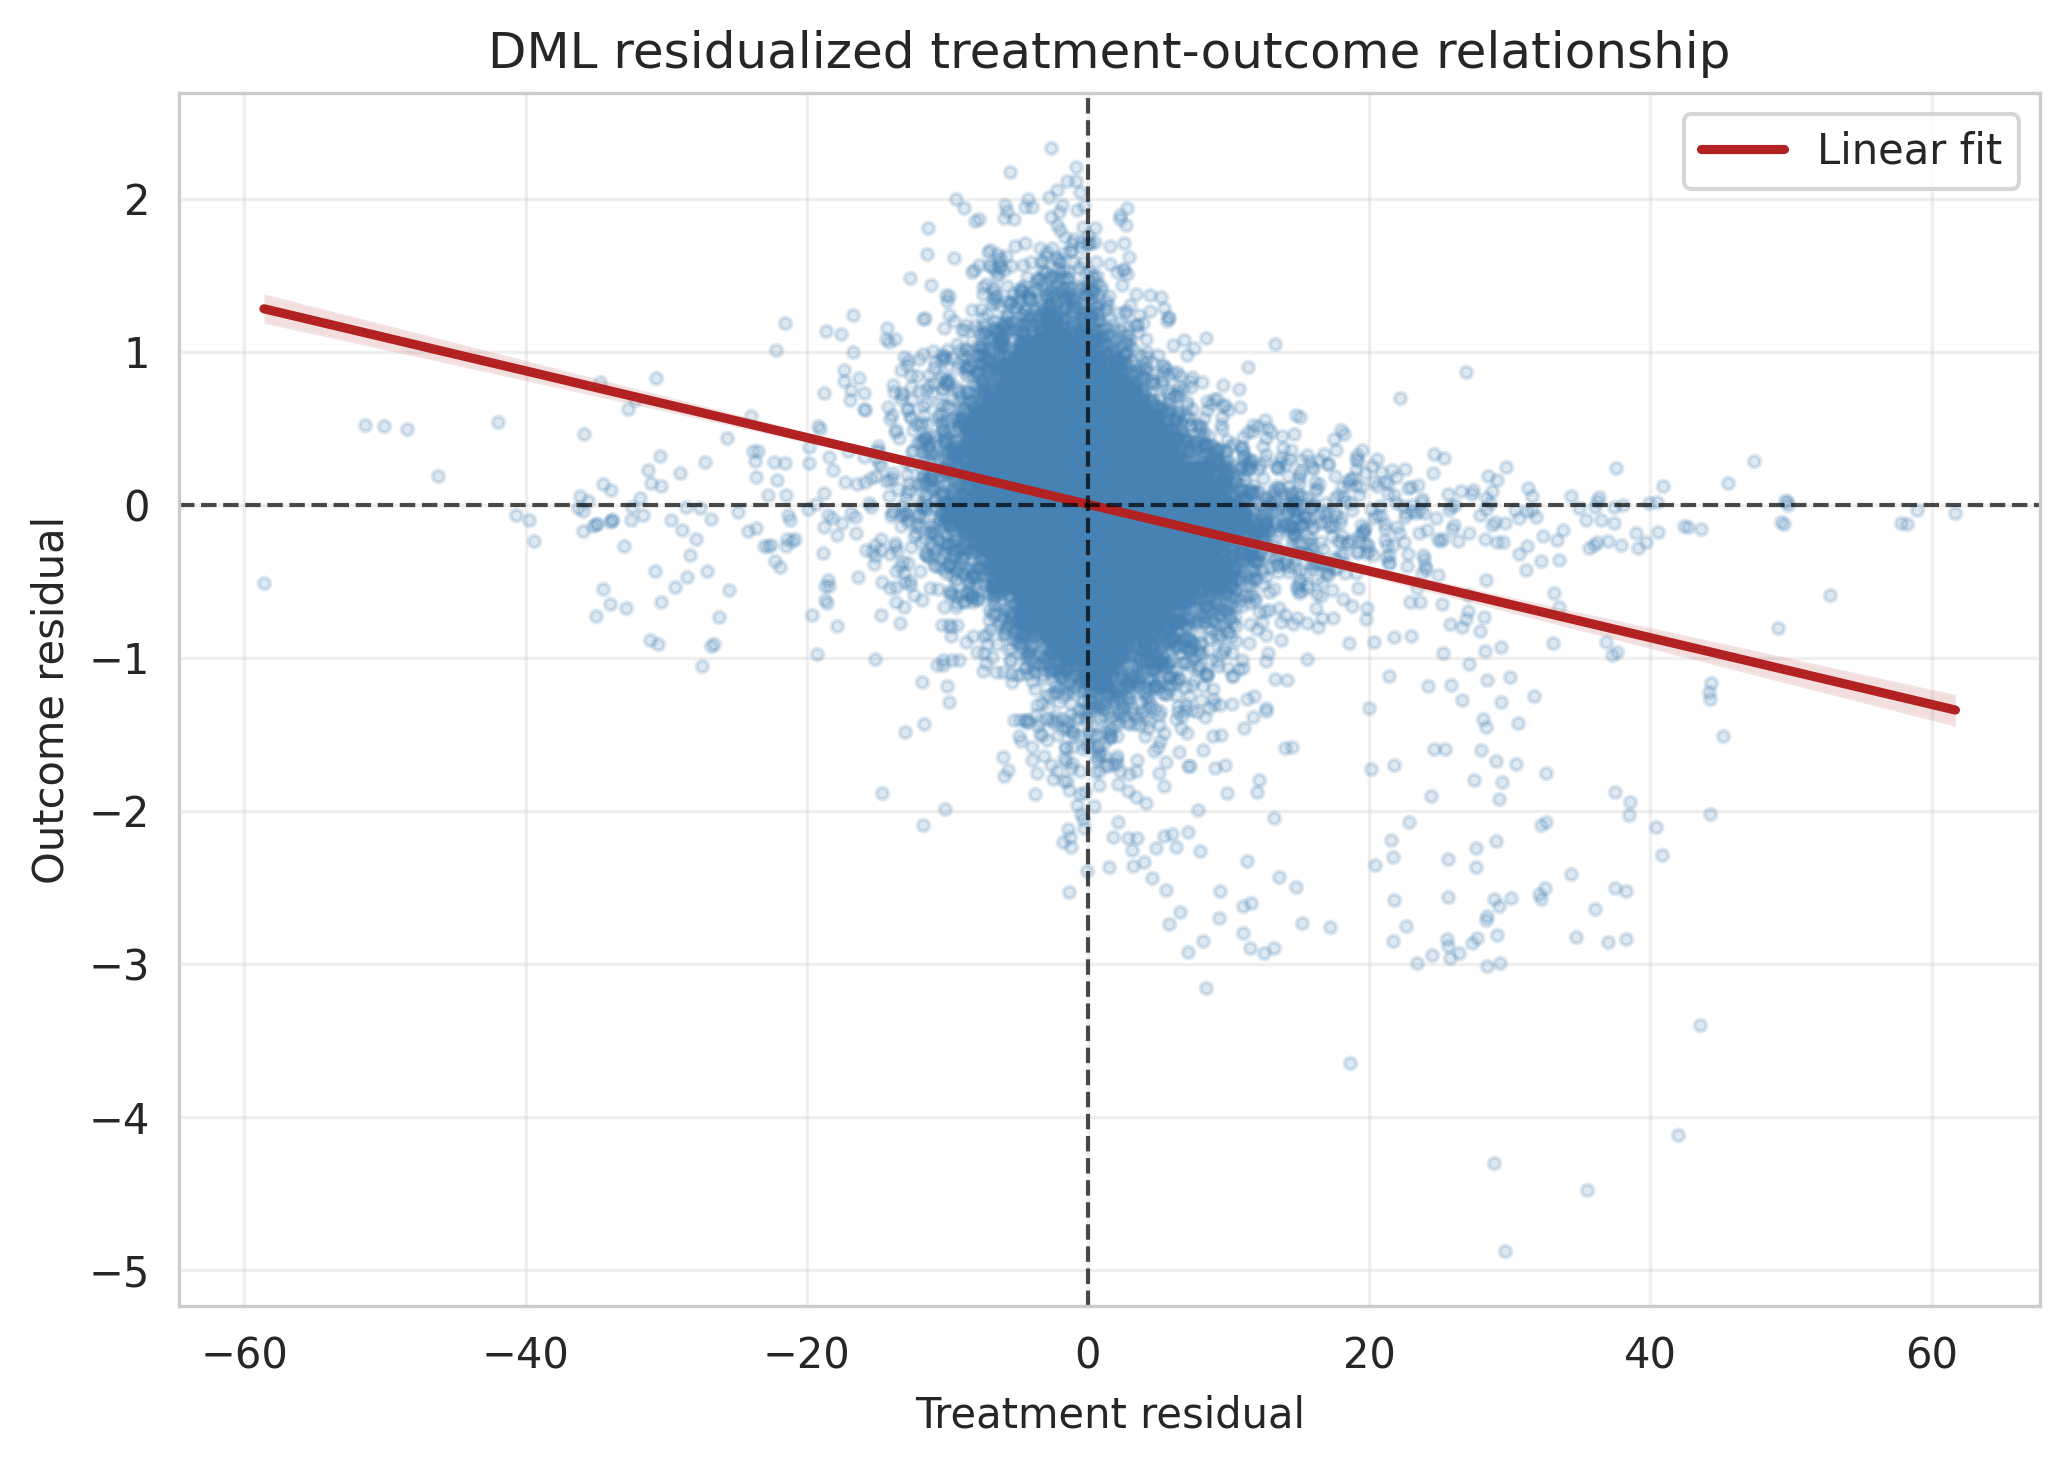
\includegraphics[width=0.78\textwidth]{Figures/dml_residualized_treatment_outcome_linear.png}}{\fbox{\parbox{0.78\textwidth}{\centering Add \texttt{dml\_residualized\_treatment\_outcome\_linear.png} to the \texttt{Figures} folder.}}}
\caption{Residualized treatment-outcome relationship after controlling for pre-pricing covariates with Double Machine Learning. The negative fitted slope is consistent with the expected demand response to higher prices.}
\label{fig:dml-residualized-linear}
\end{figure}

\begin{figure}[htbp]
\centering
\IfFileExists{Figures/cate_sales_spec_grid.png}{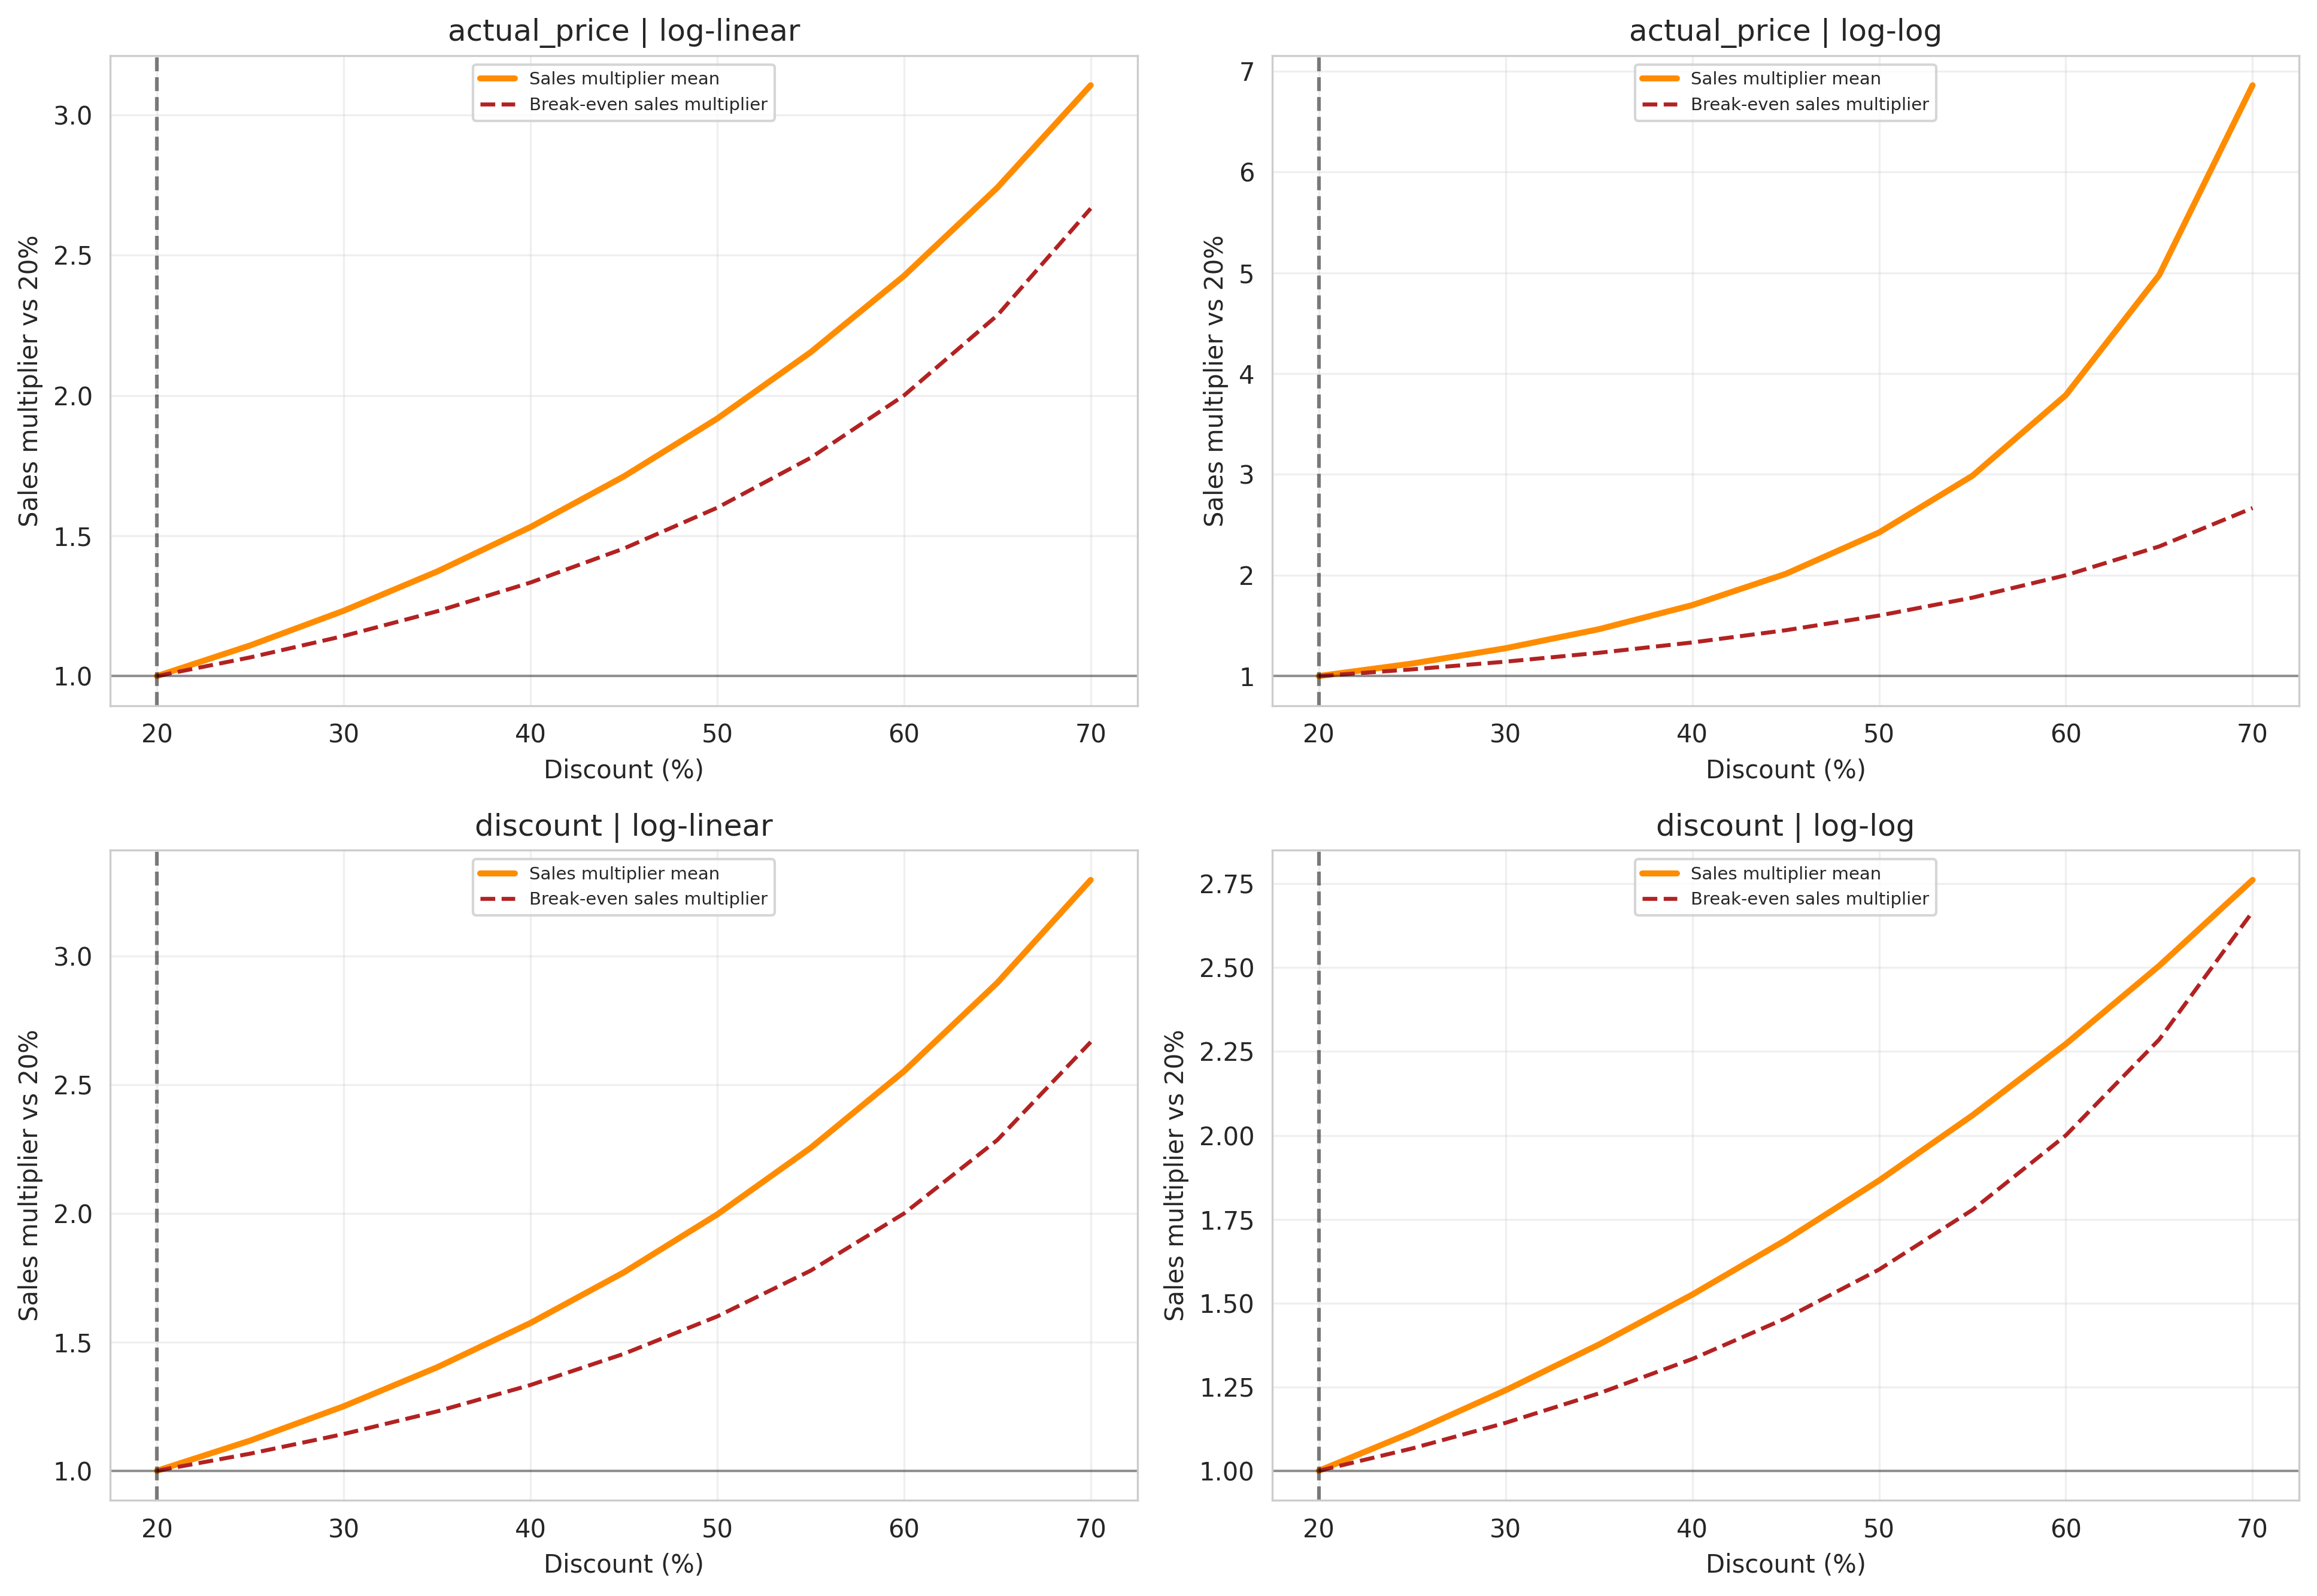
\includegraphics[width=0.95\textwidth]{Figures/cate_sales_spec_grid.png}}{\fbox{\parbox{0.95\textwidth}{\centering Add \texttt{cate\_sales\_spec\_grid.png} to the \texttt{Figures} folder.}}}
\caption{CATE-based comparison of treatment encoding and functional form. The log-linear specification using discounted price produces smoother and more economically reasonable sales-response curves than log-log or discount-based alternatives.}
\label{fig:cate-sales-spec-grid}
\end{figure}

Figure~\ref{fig:cate-sales-spec-grid} provides the empirical counterpart to the specification argument. The log-log specifications produce more polarized curves, while the log-linear specifications generate smoother responses with more plausible interior optima. Among the log-linear alternatives, the discounted-price specification is preferred because it is aligned with the revenue objective and because the treatment nuisance model is substantially stronger than in the discount-based specifications. The selected specification therefore combines a suitable revenue geometry with a stronger treatment nuisance model and smoother simulated response curves.

\section{CATE Estimation with Causal Forest}
\label{sec:cate-estimation}

A global $\hat{\beta}$ is useful for comparing specifications, but the optimizer needs one price-response curve per reference-week. To obtain heterogeneous effects, the residualized training data from the DML step are passed to EconML's \texttt{CausalForest}. The forest is fitted with $\tilde{Y}$ as the target, $\tilde{T}$ as the treatment, and the pre-pricing covariates $X$ as heterogeneity features.

The nuisance models are fitted outside the forest using the LightGBM residualization described in Section~\ref{sec:specification-dml}. The forest is therefore used only as the heterogeneous final stage, estimating how the residualized price effect varies across reference-weeks. Its configuration is reported in Appendix~\ref{AppendixA}.

Following the transformation introduced in Section~\ref{sec:local-effects-markdown-curves}, each local semi-elasticity is converted into a markdown curve over the operational discount grid from 20\% to 70\%, normalized at the 20\% reference discount. These reference-week-level sales multiplier curves are the causal input passed to the optimizer.

The estimated local effects are summarized in Chapter~\ref{Chapter5}, together with the global curve comparison and reference-level examples.